%% Análise Sistêmica da Linguagem na Psiquiatria

\chapter{Introdução à Análise Sistêmica}

A linguagem, como um espelho da mente humana, reflete a complexa teia de emoções, cognições e experiências que moldam nossa percepção do mundo e de nós mesmos. No contexto da psiquiatria, a linguagem se torna uma ferramenta crucial para acessar o universo interior do paciente, desvendando os segredos de sua mente e abrindo caminho para o diagnóstico e o tratamento de transtornos mentais.

\section{Motivação e Importância}

A linguagem é a chave para desvendar o mundo interno do paciente, revelando seus medos, esperanças, crenças e padrões de pensamento. Ao analisar a linguagem de forma sistemática e quantitativa, podemos ir além da superfície, identificando nuances e sutilezas que podem passar despercebidas em uma análise puramente qualitativa.

A Análise Sistêmica da Linguagem na Psiquiatria busca:
\begin{itemize}
    \item \textbf{Identificar padrões ocultos}: Revelar padrões emocionais e cognitivos subjacentes
    \item \textbf{Prevenir crises emocionais}: Monitorar a evolução das emoções ao longo do tempo
    \item \textbf{Monitorar o progresso terapêutico}: Avaliar objetivamente a evolução do paciente
    \item \textbf{Reduzir a subjetividade}: Oferecer uma abordagem mais objetiva e replicável
\end{itemize}

\chapter{Representação Vetorial de Frases e Sentenças}

\section{Definição do Espaço Vetorial Multidimensional}

Imaginemos um espaço vetorial $\mathbb{R}^n$, onde cada dimensão representa uma característica específica da linguagem. Cada frase ou sentença $F_i$ pode ser mapeada para um vetor $\vec{F}_i$ nesse espaço multidimensional:

\begin{equation}
\vec{F}_i = (v_1, v_2, v_3, v_4, v_5, v_6, v_7, v_8, v_9, v_{10})
\end{equation}

Onde as dimensões representam:
\begin{itemize}
    \item $v_1$: \textbf{Valência emocional} --- positiva a negativa
    \item $v_2$: \textbf{Excitação emocional} --- calmo a excitado
    \item $v_3$: \textbf{Dominância emocional} --- passivo a dominante
    \item $v_4$: \textbf{Complexidade sintática} --- sofisticação gramatical
    \item $v_5$: \textbf{Foco temático} --- tópicos principais
    \item $v_6$: \textbf{Intensidade afetiva} --- força da emoção
    \item $v_7$: \textbf{Polaridade} --- positiva, negativa, neutra
    \item $v_8$: \textbf{Coerência narrativa} --- fluidez e consistência
    \item $v_9$: \textbf{Perspectiva temporal} --- passado, presente, futuro
    \item $v_{10}$: \textbf{Dissonância cognitiva} --- discrepâncias internas
\end{itemize}

\section{Medidas de Similaridade e Divergência}

O \textbf{produto escalar} entre dois vetores mede a similaridade:

\begin{equation}
\vec{F}_i \cdot \vec{F}_j = \sum_{k=1}^{10} v_{ki} \cdot v_{kj}
\end{equation}

A \textbf{distância euclidiana} mede a divergência:

\begin{equation}
d(\vec{F}_i, \vec{F}_j) = \sqrt{\sum_{k=1}^{10} (v_{ki} - v_{kj})^2}
\end{equation}

\begin{center}
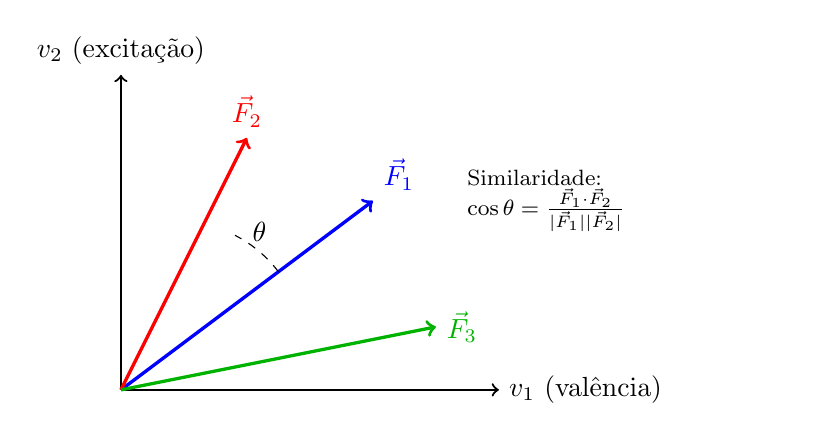
\begin{tikzpicture}[scale=0.8]
    % Eixos
    \draw[thick, ->] (0,0) -- (6,0) node[right] {$v_1$ (valência)};
    \draw[thick, ->] (0,0) -- (0,5) node[above] {$v_2$ (excitação)};

    % Vetores de frases
    \draw[very thick, ->, blue] (0,0) -- (4,3) node[above right] {$\vec{F}_1$};
    \draw[very thick, ->, red] (0,0) -- (2,4) node[above] {$\vec{F}_2$};
    \draw[very thick, ->, green!70!black] (0,0) -- (5,1) node[right] {$\vec{F}_3$};

    % Ângulo
    \draw[dashed] (2.5,1.875) arc (37:63:2);
    \node at (2.2,2.5) {$\theta$};

    % Legenda
    \node[font=\footnotesize, text width=4cm] at (8,3) {Similaridade:\\$\cos\theta = \frac{\vec{F}_1 \cdot \vec{F}_2}{|\vec{F}_1||\vec{F}_2|}$};
\end{tikzpicture}
\end{center}

\chapter{Sistema de Equações Dinâmicas Acopladas}

A interação entre estados emocionais e cognitivos pode ser descrita por um sistema de equações diferenciais acopladas:

\begin{align}
\frac{d\vec{E}(t)}{dt} &= A_E \cdot \vec{E}(t) + B_E \cdot \vec{X}(t) + C_E \cdot \vec{C}(t) \\
\frac{d\vec{C}(t)}{dt} &= A_C \cdot \vec{C}(t) + B_C \cdot \vec{Y}(t) + C_C \cdot \vec{E}(t)
\end{align}

Onde:
\begin{itemize}
    \item $\vec{E}(t)$: Vetor do estado emocional no tempo $t$
    \item $\vec{C}(t)$: Vetor do estado cognitivo no tempo $t$
    \item $A_E, A_C$: Matrizes de dinâmica interna
    \item $B_E, B_C$: Matrizes de influência externa
    \item $C_E, C_C$: Matrizes de acoplamento mútuo
\end{itemize}

\begin{center}
\begin{tikzpicture}[scale=1]
    \node[draw, ellipse, fill=red!20, minimum width=3cm, minimum height=1.5cm] (E) at (-3,0) {Estado Emocional $\vec{E}$};
    \node[draw, ellipse, fill=blue!20, minimum width=3cm, minimum height=1.5cm] (C) at (3,0) {Estado Cognitivo $\vec{C}$};

    \draw[very thick, <->, purple] (E) -- node[above] {$C_E, C_C$} (C);

    \node[draw, rounded corners, fill=orange!20] (X) at (-3,-3) {Estímulos $\vec{X}$};
    \node[draw, rounded corners, fill=green!20] (Y) at (3,-3) {Estímulos $\vec{Y}$};

    \draw[thick, ->] (X) -- node[left] {$B_E$} (E);
    \draw[thick, ->] (Y) -- node[right] {$B_C$} (C);

    % Autoloops
    \draw[thick, ->] (E.north) to[out=120,in=60,looseness=4] node[above] {$A_E$} (E.north);
    \draw[thick, ->] (C.north) to[out=120,in=60,looseness=4] node[above] {$A_C$} (C.north);
\end{tikzpicture}
\end{center}

\chapter{Superfície Geométrica da Linguagem e Emoção}

A superfície $S(x, y, t)$ representa a evolução dos estados emocionais e cognitivos:

\begin{equation}
S(x, y, t) = f(v(t), e(t), d(t), c(t))
\end{equation}

O \textbf{gradiente} indica a direção de maior variação:

\begin{equation}
\nabla S(x, y, t) = \left(\frac{\partial S}{\partial x}, \frac{\partial S}{\partial y}, \frac{\partial S}{\partial t}\right)
\end{equation}

A \textbf{curvatura} mede a intensidade das mudanças:

\begin{equation}
\kappa(t) = \frac{|\nabla S'(t) \times \nabla S''(t)|}{|\nabla S(t)|^3}
\end{equation}

\begin{center}
\begin{tikzpicture}[scale=0.7]
    % Superfície 3D simplificada
    \draw[thick, ->] (0,0) -- (6,0) node[right] {Valência};
    \draw[thick, ->] (0,0) -- (0,5) node[above] {Excitação};
    \draw[thick, ->] (0,0) -- (-2,-2) node[below left] {Tempo};

    % Curva na superfície
    \draw[very thick, blue, smooth] plot coordinates {
        (1,1) (2,2.5) (3,2) (4,3.5) (5,3)
    };

    % Gradiente
    \draw[thick, ->, red] (3,2) -- (4,3) node[right] {$\nabla S$};

    % Ponto de curvatura alta
    \fill[orange] (2,2.5) circle (0.15);
    \node[font=\tiny, above] at (2,2.7) {alta $\kappa$};
\end{tikzpicture}
\end{center}

\chapter{Transformada de Fourier na Análise de Linguagem}

A Transformada de Fourier decompõe o sinal da linguagem em componentes de frequência:

\begin{equation}
F(\omega) = \int_{-\infty}^{+\infty} L(t) e^{-i\omega t} \, dt
\end{equation}

Onde:
\begin{itemize}
    \item $L(t)$: Sinal da linguagem no tempo
    \item $F(\omega)$: Componentes de frequência
    \item $\omega$: Frequência angular
\end{itemize}

\begin{center}
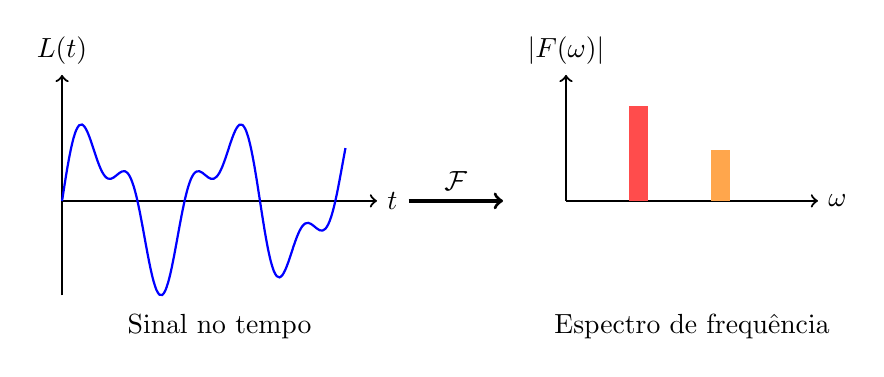
\begin{tikzpicture}[scale=0.8]
    % Sinal no tempo
    \begin{scope}
        \draw[thick, ->] (0,0) -- (5,0) node[right] {$t$};
        \draw[thick, ->] (0,-1.5) -- (0,2) node[above] {$L(t)$};
        \draw[thick, blue, smooth, samples=100, domain=0:4.5]
            plot (\x, {sin(3*\x r) + 0.5*sin(7*\x r)});
        \node at (2.5,-2) {Sinal no tempo};
    \end{scope}

    % Seta de transformação
    \draw[very thick, ->] (5.5,0) -- (7,0) node[midway, above] {$\mathcal{F}$};

    % Espectro de frequência
    \begin{scope}[shift={(8,0)}]
        \draw[thick, ->] (0,0) -- (4,0) node[right] {$\omega$};
        \draw[thick, ->] (0,0) -- (0,2) node[above] {$|F(\omega)|$};
        \fill[red!70] (1,0) rectangle (1.3,1.5);
        \fill[orange!70] (2.3,0) rectangle (2.6,0.8);
        \node at (2,-2) {Espectro de frequência};
    \end{scope}
\end{tikzpicture}
\end{center}

\chapter{Modelo Polinomial para Carga Cognitiva}

A carga cognitiva $C(x)$ como função da complexidade $x$:

\begin{equation}
C(x) = a_n x^n + a_{n-1} x^{n-1} + \cdots + a_1 x + a_0
\end{equation}

A derivada indica a taxa de variação:

\begin{equation}
C'(x) = n a_n x^{n-1} + (n-1) a_{n-1} x^{n-2} + \cdots + a_1
\end{equation}

\begin{center}
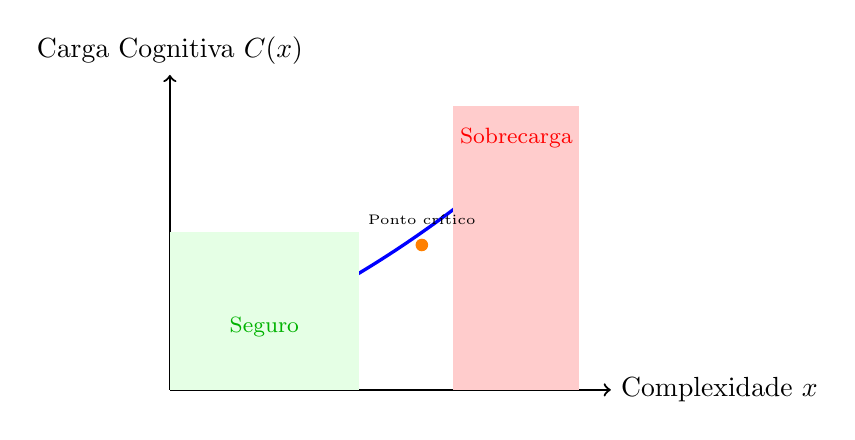
\begin{tikzpicture}[scale=0.8]
    \draw[thick, ->] (0,0) -- (7,0) node[right] {Complexidade $x$};
    \draw[thick, ->] (0,0) -- (0,5) node[above] {Carga Cognitiva $C(x)$};

    % Curva polinomial
    \draw[very thick, blue, smooth, samples=100, domain=0.5:6]
        plot (\x, {0.05*\x*\x + 0.3*\x + 0.5});

    % Zona de sobrecarga
    \fill[red!20] (4.5,0) rectangle (6.5,4.5);
    \node[font=\footnotesize, red] at (5.5,4) {Sobrecarga};

    % Zona segura
    \fill[green!10] (0,0) rectangle (3,2.5);
    \node[font=\footnotesize, green!70!black] at (1.5,1) {Seguro};

    % Ponto crítico
    \fill[orange] (4,2.3) circle (0.1);
    \node[font=\tiny] at (4,2.7) {Ponto crítico};
\end{tikzpicture}
\end{center}

\section{Aplicações Clínicas}

\begin{enumerate}
    \item \textbf{Diagnóstico mais preciso}: Identificar padrões linguísticos sutis
    \item \textbf{Prevenção de crises}: Monitorar evolução emocional em tempo real
    \item \textbf{Personalização do tratamento}: Ajustar intervenções individualmente
    \item \textbf{Avaliação objetiva do progresso}: Medir evolução com precisão
\end{enumerate}

\begin{sintese}[title=Síntese da Análise Sistêmica]
A Análise Sistêmica da Linguagem na Psiquiatria representa um passo audacioso em direção a uma compreensão mais profunda e objetiva da mente humana. Ao combinar a riqueza da linguagem com o poder das ferramentas matemáticas e computacionais, abrimos novas portas para o diagnóstico, o tratamento e o cuidado da saúde mental, oferecendo esperança e novas possibilidades para pacientes e profissionais da área.
\end{sintese}

\nextpage
